\documentclass{bioinfo}
\copyrightyear{2014}
\pubyear{2014}

\usepackage{hyperref}

\begin{document}
\firstpage{1}

%\title[short Title]{Structure prediction of globular proteins using predicted residue contacts.}
%\title[short Title]{PconsFold: ab-initio protein folding using Rosetta and predicted residue contacts.}
\title[short Title]{PconsFold: Protein folding using predicted residue contacts.}
%\title[short Title]{Advancement in residue contact prediction improves quality of predicted structural models.}
%\author[Sample \textit{et~al}]{Mirco Michel\,$^{1,2}$, Marcin J. Skwark\,$^{3}$ and Arne Elofsson\,$^{1,2}$\footnote{to whom correspondence should be addressed}}
\author[Sample \textit{et~al}]{Mirco Michel\,$^{1,2}$ and Arne Elofsson\,$^{1,2}$\footnote{to whom correspondence should be addressed}}
\address{$^{1}$Department of Biochemistry and Biophysics, Stockholm University, 10691 Stockholm, Sweden\\
$^{2}$Science for Life Laboratory, Box 1031, 17121 Solna, Sweden}
%$^{3}$Department of Information and Computer Science, Helsinki University of Technology TKK, Box 5400, FI-02015 TKK, Finland}

\history{Received on XXXXX; revised on XXXXX; accepted on XXXXX}

\editor{Associate Editor: XXXXXXX}

\maketitle

\begin{abstract}

\section{Motivation:}

\section{Results:}
Here we show that improved quality of evolutionary constraints increases quality and native-likeliness of predicted models. We also show that 
\section{Availability:}
We provide a fully automated pipeline, PconsFold, for predicting protein structures based on evolutionary information. PconsFold is based on PconsC and Rosetta and freely available at \url{https://github.com/ElofssonLab/pcons-fold}.
\section{Contact:} \href{arne@bioinfo.se}{arne@bioinfo.se}
\end{abstract}

\section{Introduction}
Predicting protein structures from sequences is one of the longest standing problems in structural biology. Although the problem itself remains unsolved, there has been continous effort and progress resulting in increased accuracy of predicted models \cite{casp}. 
Here we show that improved quality of evolutionary constraints increases quality and native-likeliness of predicted models. We elucidate diverging folding performance over different fold-classes. 
Structure prediction ab-initio still hard / motivate using sequence information to help structure prediction / residue contact map prediction improved dramatically / large amount of available sequences allows to use global models (DCA) instead of local models (MI) / now predicted contacts are precise enough to fascilitate ab-initio structure prediction / But what is the best way to do that? \\ 
Here we introduce a Rosetta folding protocol that uses residue contacts and includes these into the energy function / We benchmark our method on different datasets (PSICOV, Marks et al. 2013 and CASP10), CNS and Fragfold / We compare our method to other methods (CNS and Fragfold) / With our method we then predict the structure of all Pfam domains with previously unknown structure and enough available sequence data / 

\section{Approach}
Predicted contacts are used to constrain folding space / included in energy functions of Rosetta \& CNS \& Fragfold(?) / Benchmarked on different datasets(PSICOV, Marks et al. 2013, CASP10) / by calculating TM-scores of the top ranked models to the native structures / we investigate how many predicted contacts are needed for each method to attain highest accuracy / we optimize our Rosetta protocol in terms of runtime and accuracy / 

\begin{methods}
\section{Methods}
\begin{figure}[!tpb]%figure1
    \centerline{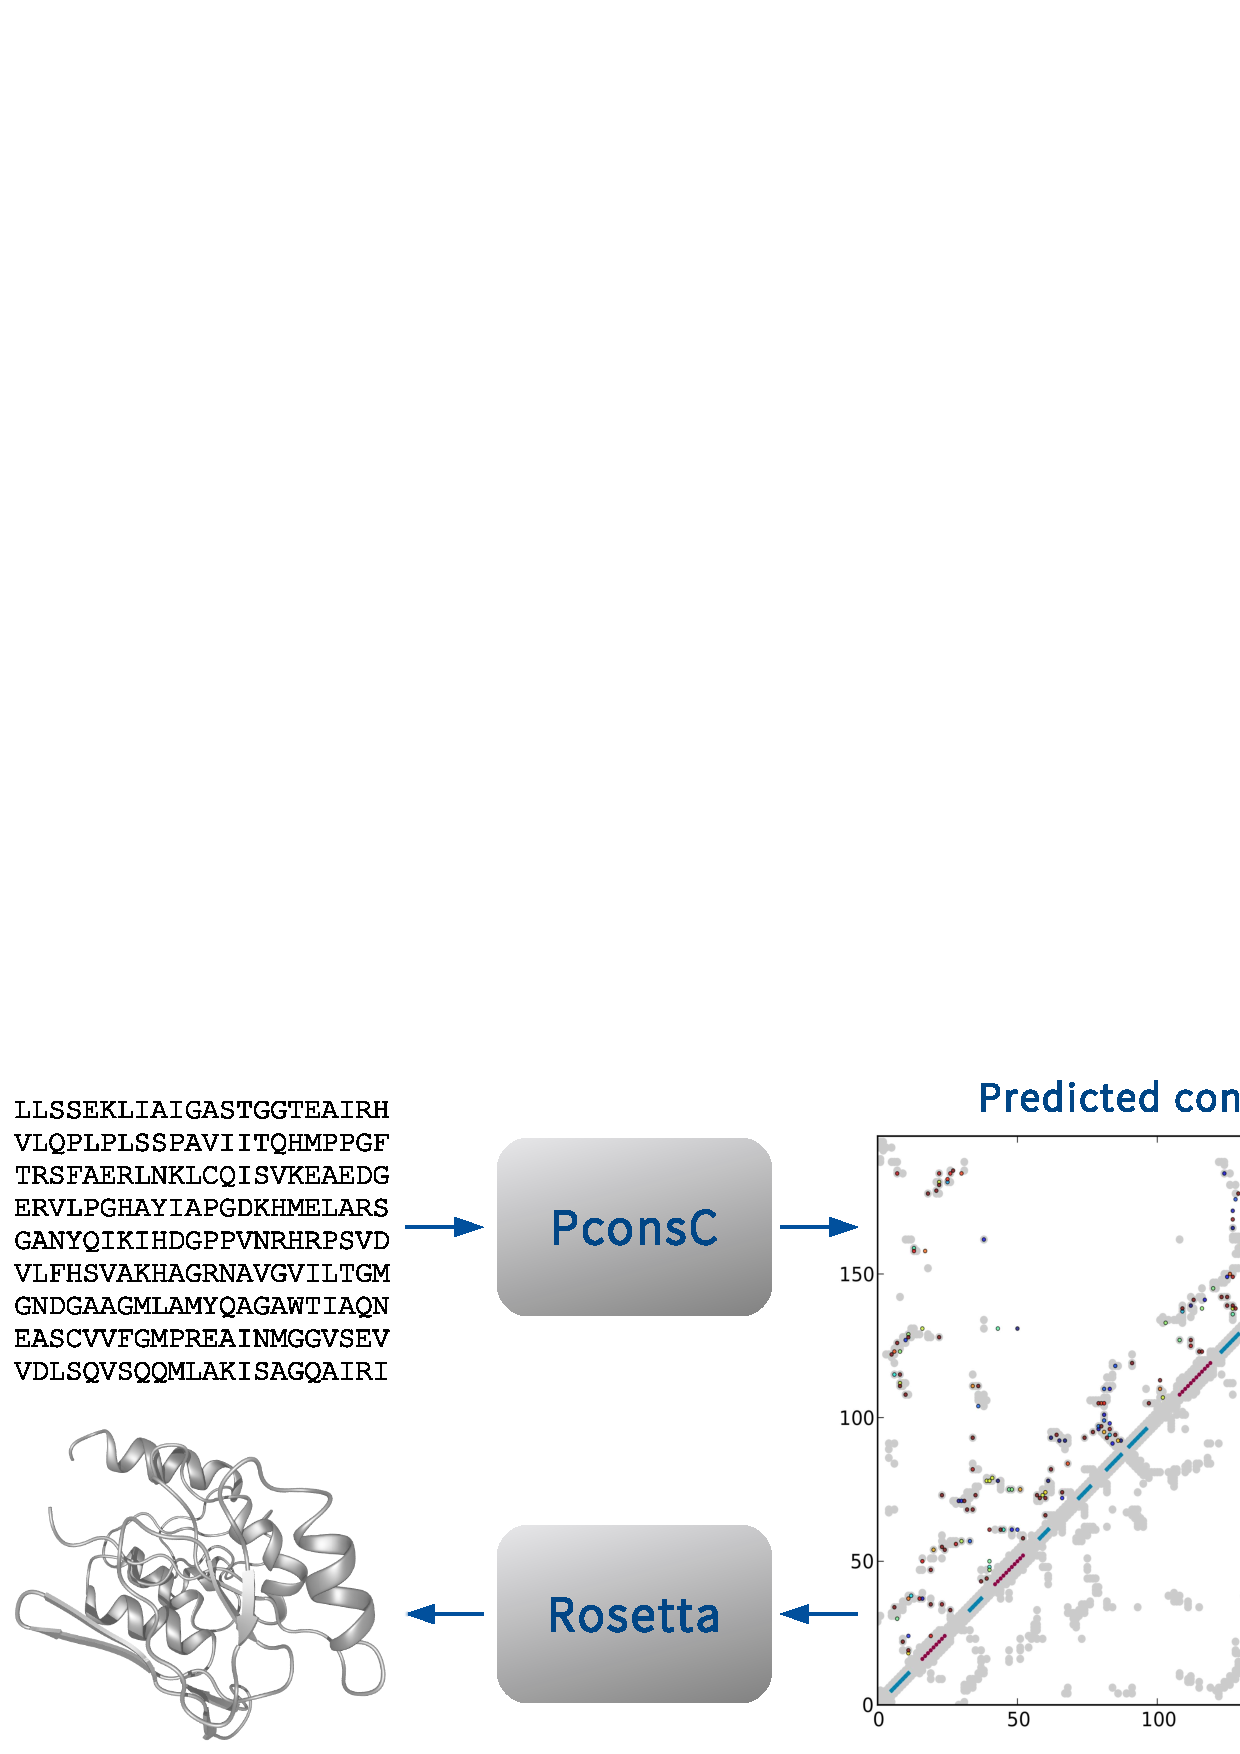
\includegraphics[scale=0.37]{figures/pipeline.png}}
\caption{PconsFold pipeline.}\label{fig:main}
\end{figure}
Rosetta: Fragment replacement by Markov chain Monte Carlo simulation / starting from extended amino acid chain / iteratively changing backbone dihedrals of parts of the chain according to selected fragment / calculate energy of the new conformation, then keep or dismiss it / works without residue contact information, but very slow convergence and only feasible for very small proteins / dramatic reduction in computational time when including contact information / therefore also applicable to larger proteins and more comprehensive studies possible (e.g. Pfam domain prediction) / \\
CNS: Very fast / standard tool for protein structure determination by NMR / folds the protein using only contact and secondary structure information / thus, truly de-novo folding / What is the energy function / How is contact information exactly incorporated \\
Fragfold: Similar approach than Rosetta / stochastic exploration of folding space by fragment replacement / however, different philosophy behind the approach / Whereas Rosetta focusses on quickly generating a lot of rough models to sample structural space, Fragfold focusses on generating few models, but with a lot more refinement / Fragfold explores the structural space more extensively within a single run / Thus one run takes much longer than with Rosetta / 


\end{methods}
\section{Results}
Fig.\ \ref{fig:main}: How many contacts to use? Elucidate differences between the methods \\
Fig.\ \ref{fig:ros}: How strongly to weight them in Rosetta? \\
Fig.\ \ref{fig:vs}: How many Rosetta decoys are needed to get close to the native structure? How low can we go without loosing too much accuracy? \\
What can we say about the quality of our Pfam domain models: \\

\begin{figure}[!tpb]%figure1
    \centerline{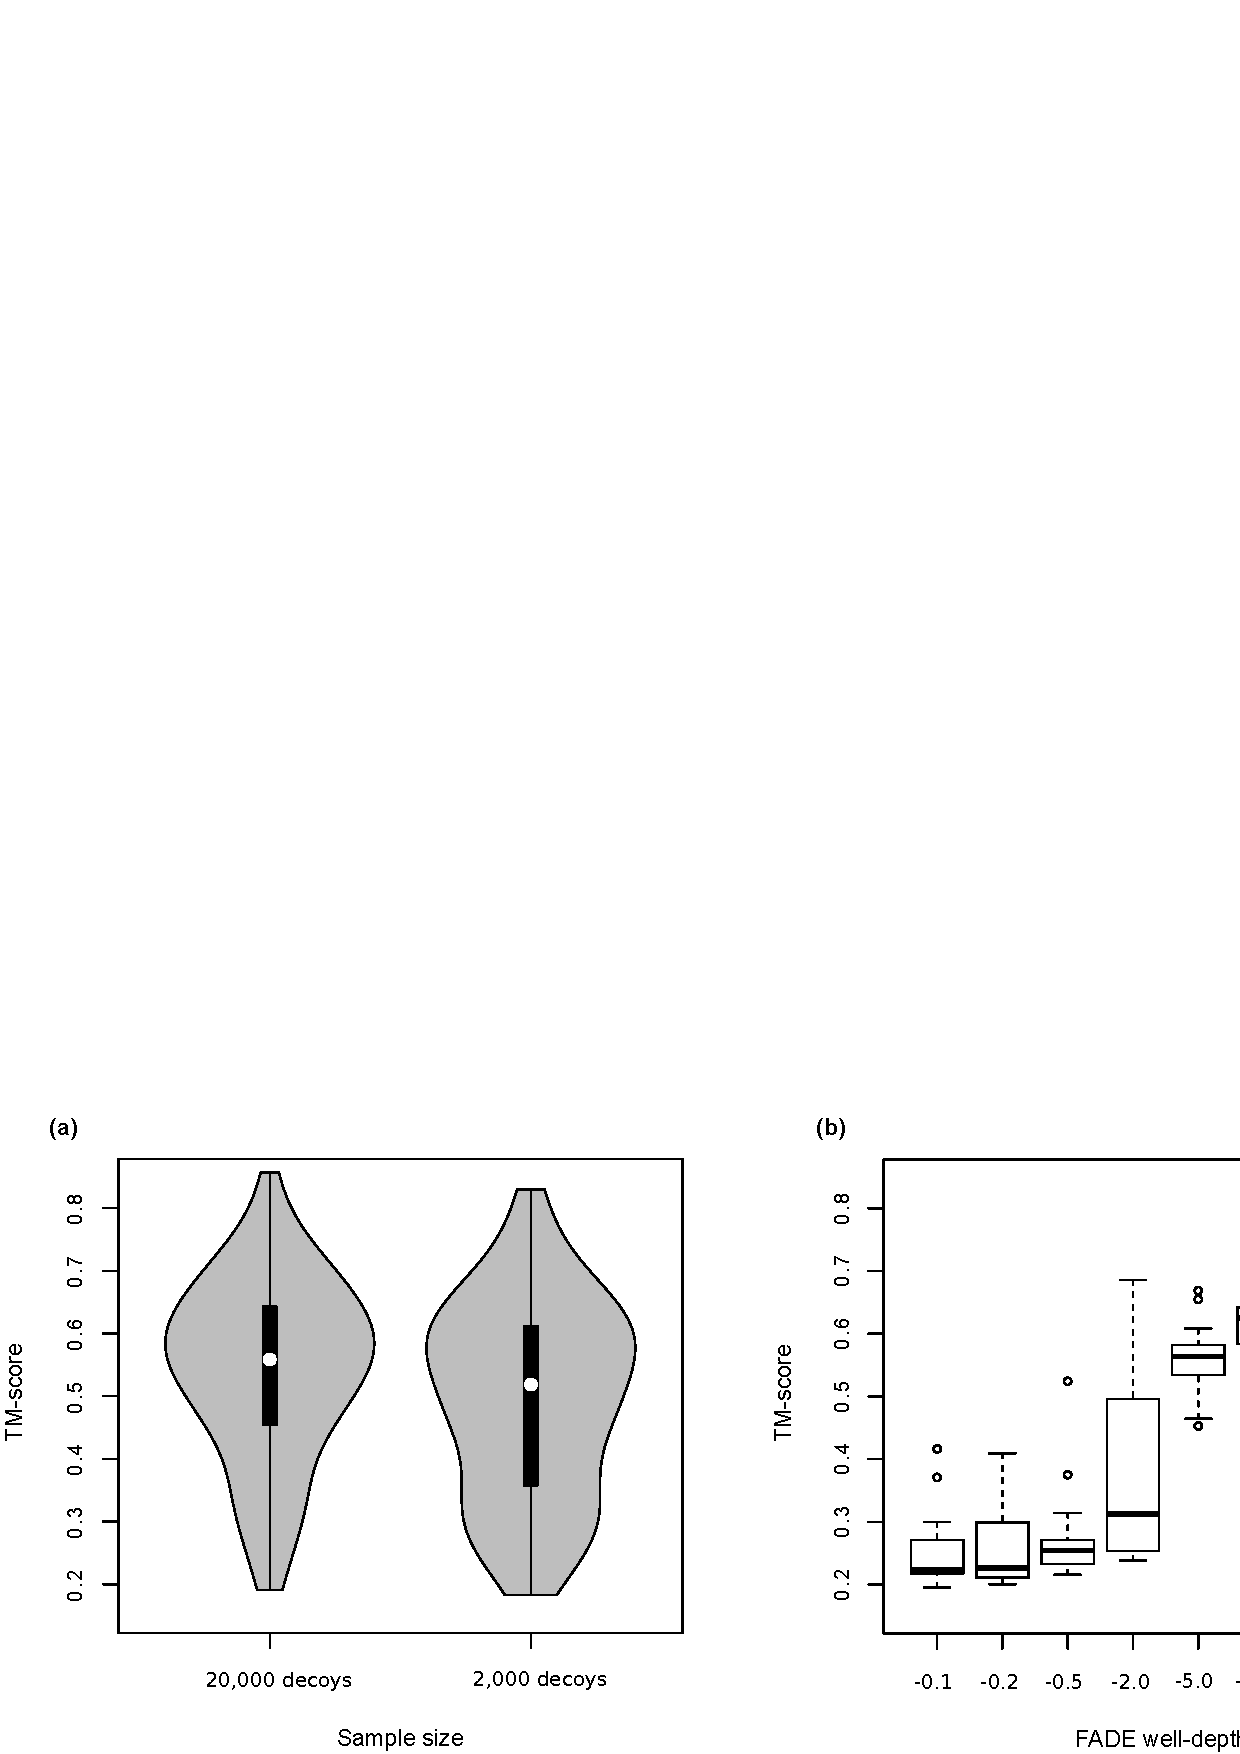
\includegraphics[scale=1.0]{figures/rosetta.png}}
\caption{Average TM-scores.}\label{fig:ros}
\end{figure}

\begin{figure}[!tpb]%figure1
    \centerline{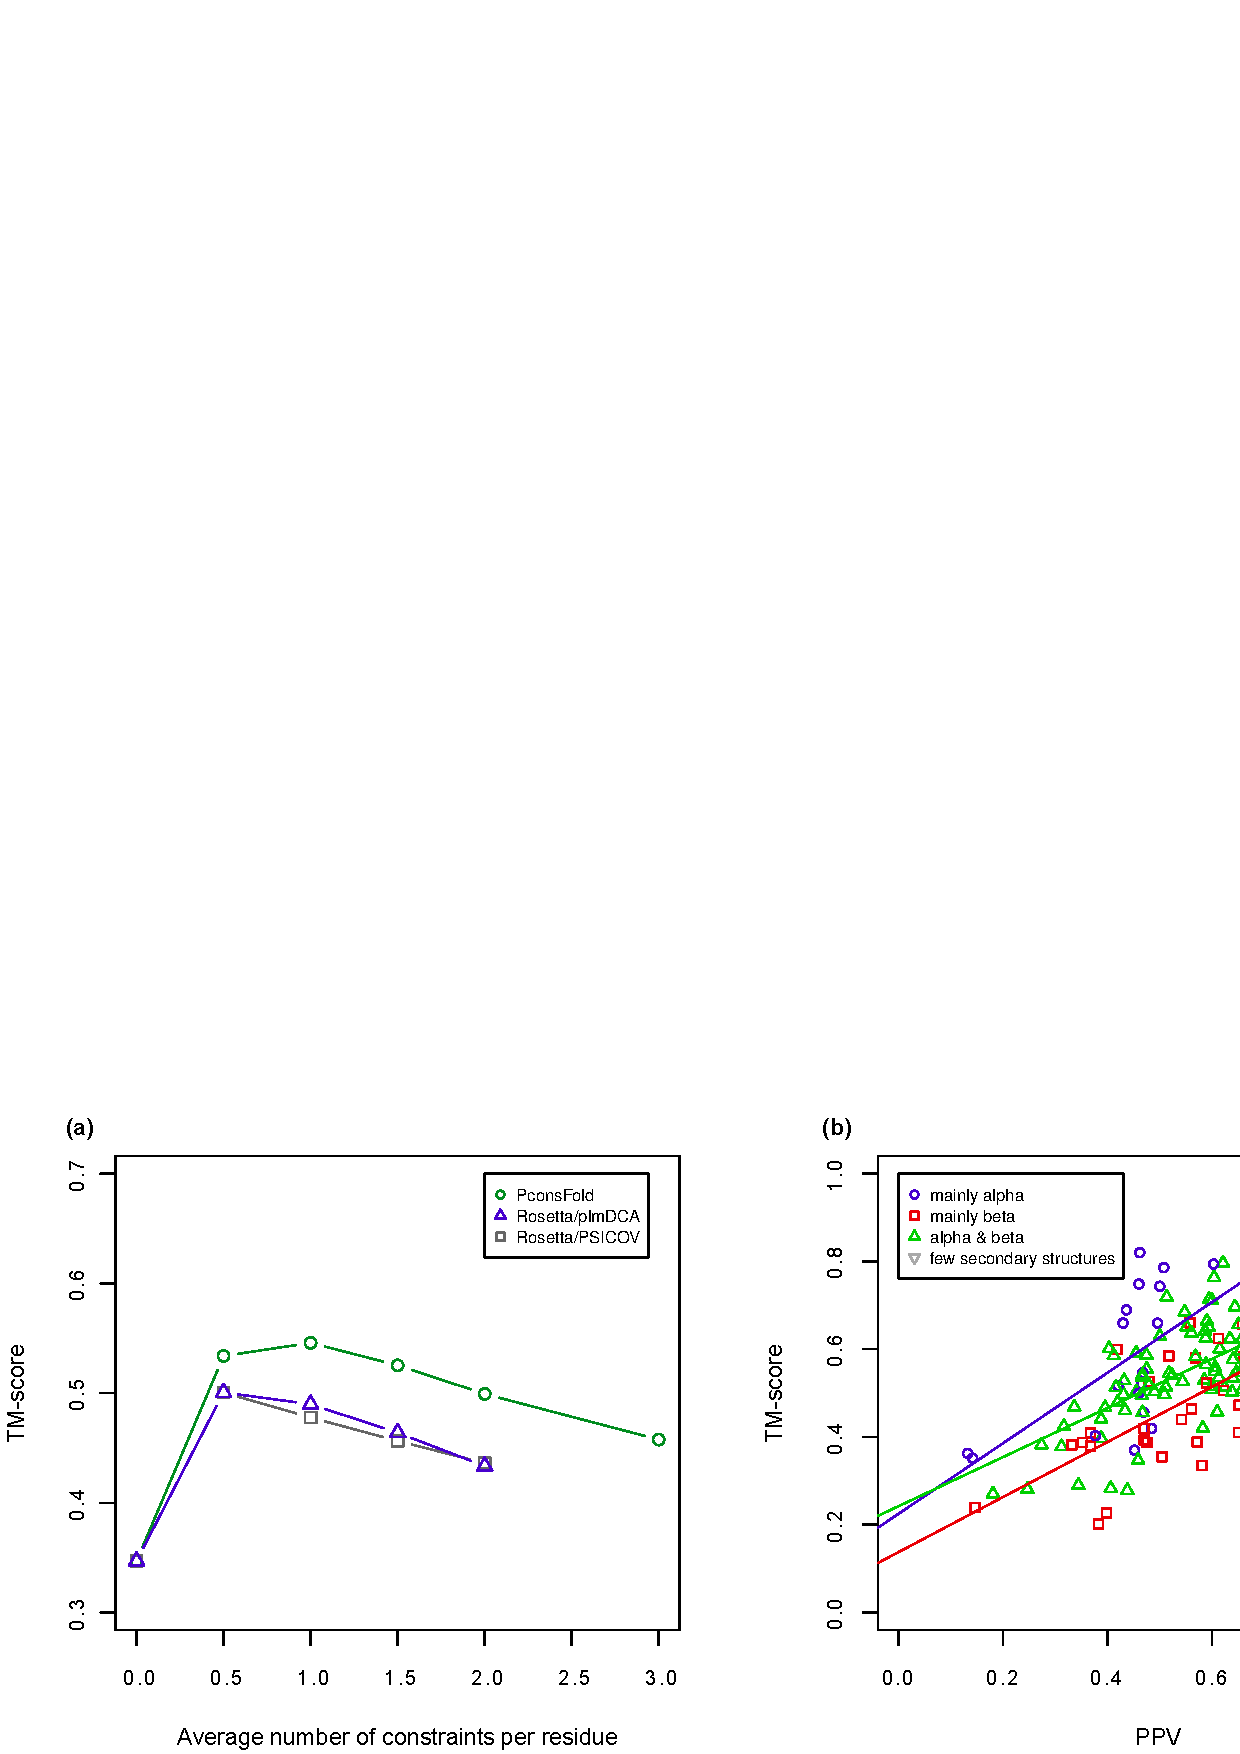
\includegraphics[scale=1.0]{figures/tmscores.png}}
\caption{(a) Average TM-scores. (b) TM-scores against PPV of underlying contact maps.}\label{fig:main}
\end{figure}

\begin{table}[!t]
\processtable{Average TM-scores for different QA tools\label{tab:qa}}
{\begin{tabular}{llll}\toprule
    Method  & EVfold & PconsFold & Rosetta/plmDCA \\ \midrule
    Rosetta & --     & 0.55     & 0.5          \\
    Pcons   & 0.47  & 0.53     & 0.47          \\
    Proq2   & 0.36  & 0.51     & 0.46          \\
    DOPE    & 0.46  & 0.36     & ~              \\ \botrule
\end{tabular}}{}
\end{table}

\begin{figure}[!tpb]%figure1
    \centerline{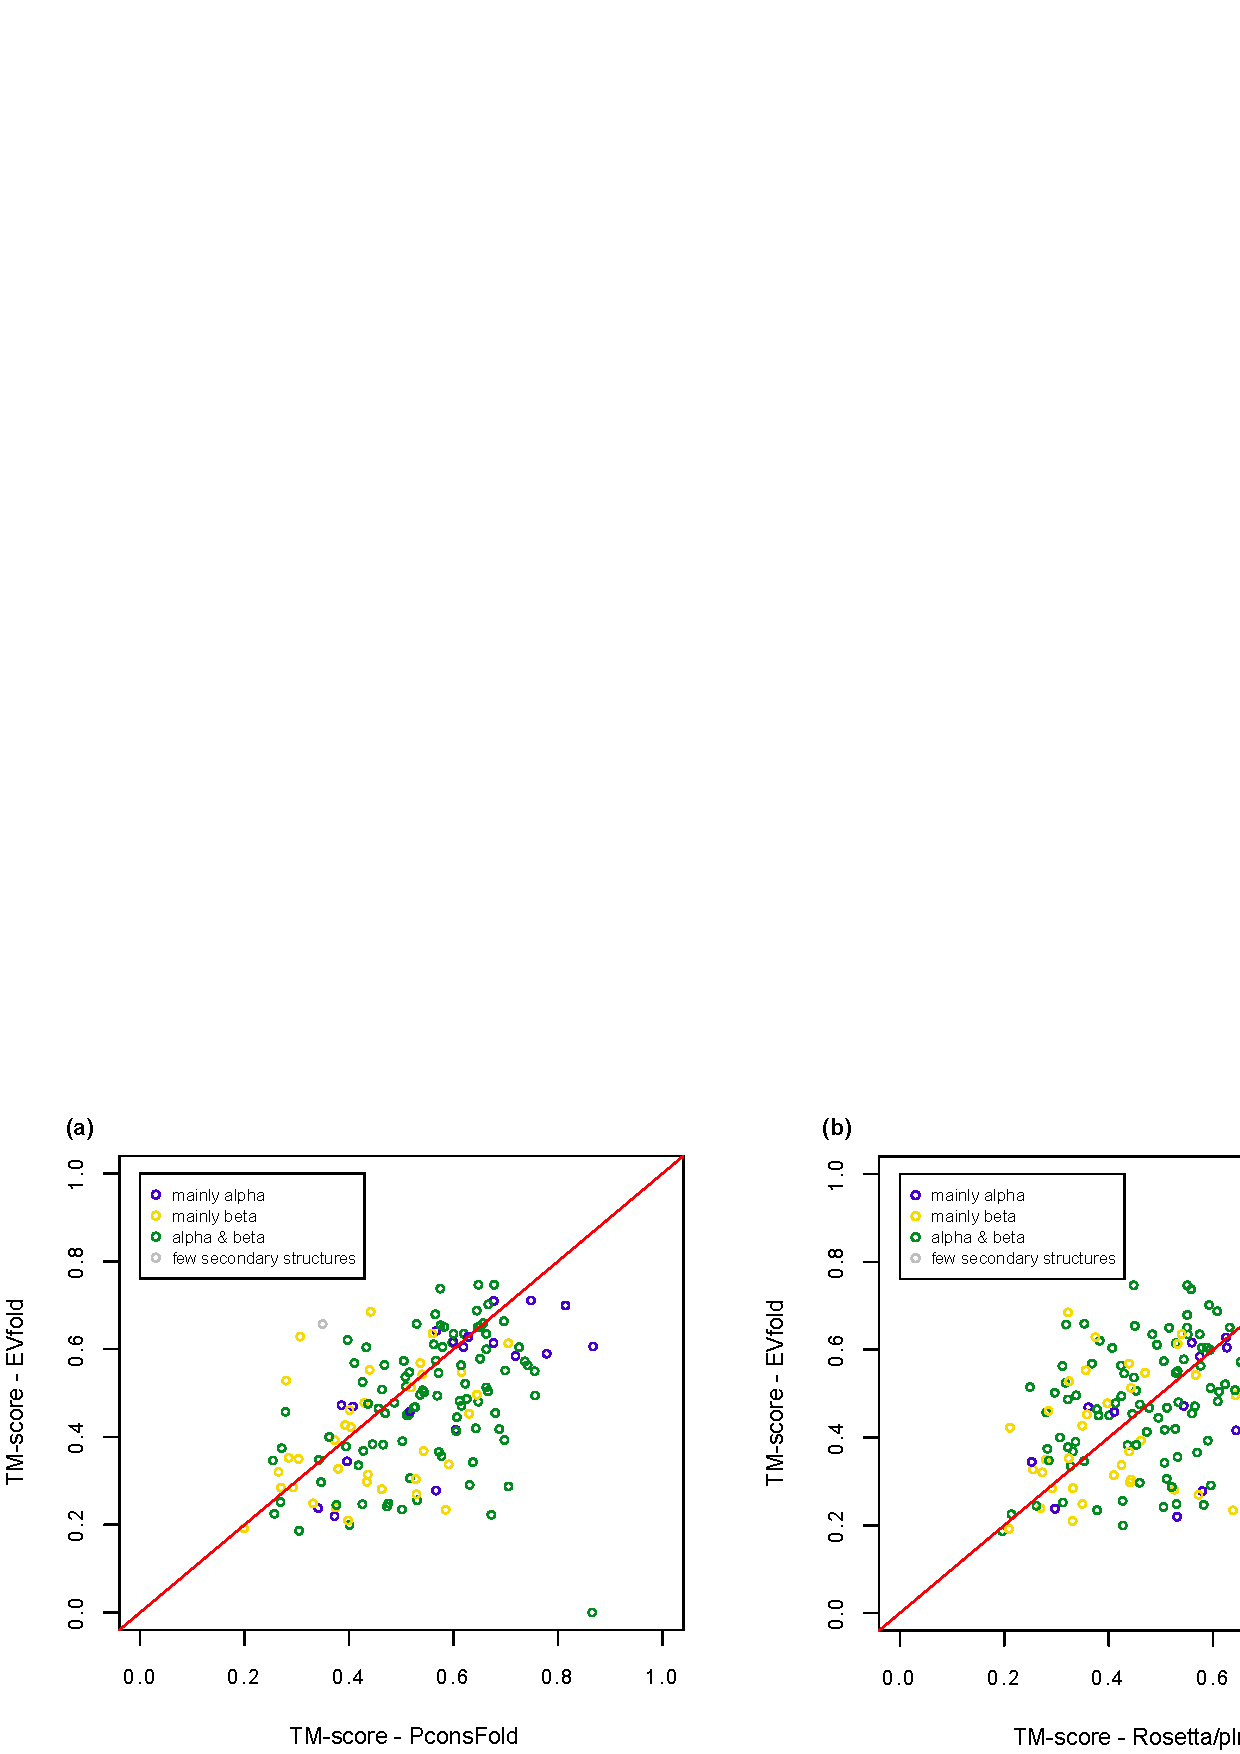
\includegraphics[scale=1.0]{figures/vs.png}}
\caption{PconsFold compared to EVfold.}\label{fig:vs}
\end{figure}

\begin{table}[!t]
\processtable{TM-scores for top ranked models. OLD (needs to be redone with selected QA)\label{tab:evfold}}
{\begin{tabular}{cccc}\toprule
    Protein      & EVfold (paper) & EVfold (web) & PconsFold \\ \midrule
    BPT1\_BOVIN  & 0.49   & 0.25           & 0.65      \\
    CADH1\_HUMAN & 0.55   & 0.54           & 0.54      \\
    CD209\_HUMAN & 0.39   & 0.64           & 0.54      \\
    CHEY\_ECOLI  & 0.65   & 0.66           & 0.83      \\
    ELAV4\_HUMAN & 0.57   & 0.61           & 0.5       \\
    O45418\_CAEEL & 0.48   & 0.62           & 0.28      \\
    OMPR\_ECOLI  & 0.35   & 0.44           & 0.48      \\
    OPSD\_BOVIN  & 0.5    & 0.55           & 0.55      \\
    PCB1\_HUMAN  & 0.25   & 0.43           & 0.43      \\
    RASH\_HUMAN  & 0.7    & 0.62           & 0.75      \\
    RNH\_ECOLI   & 0.54   & 0.66           & 0.62      \\
    SPTB2\_HUMAN & 0.37   & 0.51           & 0.6       \\
    THIO\_ALIAC  & 0.55   & 0.56           & 0.76      \\
    TRY2\_RAT    & 0.53*  & 0.78           & 0.83      \\
    YES\_HUMAN   & 0.35   & 0.31           & 0.55      \\ \midrule
    Mean         & 0.48   & 0.55           & 0.59      \\ \botrule
\end{tabular}}{}
\end{table}

\section{Conclusion}


\section*{Acknowledgement}
%Text Text Text Text Text Text  Text Text.  \citealp{Boffelli03} might want to know about  text text text text

\paragraph{Funding\textcolon} %Text Text Text Text Text Text  Text Text.

%\bibliographystyle{natbib}
%\bibliographystyle{achemnat}
%\bibliographystyle{plainnat}
%\bibliographystyle{abbrv}
%\bibliographystyle{bioinformatics}
%
%\bibliographystyle{plain}
%
%\bibliography{Document}


\begin{thebibliography}{}
%\bibitem[Bofelli {\it et~al}., 2000]{Boffelli03} Bofelli,F., Name2, Name3 (2003) Article title, {\it Journal Name}, {\bf 199}, 133-154.

%\bibitem[Bag {\it et~al}., 2001]{Bag01} Bag,M., Name2, Name3 (2001) Article title, {\it Journal Name}, {\bf 99}, 33-54.

%\bibitem[Yoo \textit{et~al}., 2003]{Yoo03}
%Yoo,M.S. \textit{et~al}. (2003) Oxidative stress regulated genes
%in nigral dopaminergic neurnol cell: correlation with the known
%pathology in Parkinson's disease. \textit{Brain Res. Mol. Brain
%Res.}, \textbf{110}(Suppl. 1), 76--84.

%\bibitem[Lehmann, 1986]{Leh86}
%Lehmann,E.L. (1986) Chapter title. \textit{Book Title}. Vol.~1, 2nd edn. Springer-Verlag, New York.

%\bibitem[Crenshaw and Jones, 2003]{Cre03}
%Crenshaw, B.,III, and Jones, W.B.,Jr (2003) The future of clinical
%cancer management: one tumor, one chip. \textit{Bioinformatics},
%doi:10.1093/bioinformatics/btn000.

%\bibitem[Auhtor \textit{et~al}. (2000)]{Aut00}
%Auhtor,A.B. \textit{et~al}. (2000) Chapter title. In Smith, A.C.
%(ed.), \textit{Book Title}, 2nd edn. Publisher, Location, Vol. 1, pp.
%???--???.

%\bibitem[Bardet, 1920]{Bar20}
%Bardet, G. (1920) Sur un syndrome d'obesite infantile avec
%polydactylie et retinite pigmentaire (contribution a l'etude des
%formes cliniques de l'obesite hypophysaire). PhD Thesis, name of
%institution, Paris, France.

\end{thebibliography}
\end{document}
